\paragraph{}
A different strategy might perform better in one domain and worse in another.
Our goal was to find the correlation of the domain characteristics with the performance of each of the agents in our arsenal in that domain, in order to choose the one that will theoretically give us the best utility. 

\paragraph{}
 First we needed to collect data that will give us insight about the performance of each agent in a given domain. 
 This was handled by a custom runner, that ran negotiation rounds and stored the utility in files.
 \paragraph{}
 We set a negotiation setting with 5 agents in the arsenal, 10 opponents and 45 domains, meaning approximately 4500 negotiation rounds and approximately
10 hours of runtime (split into multiple computers by running the negotiations in separate domains in the same time).
\paragraph{}
 From this data we collected the average utility (the negotiation rounds with 10 opponents ) of each of the 5 agents and the characteristics of the domain. 
 The characteristics of the domain that we used are:
\begin{itemize}
	\item {Average bid utility} 
	\item {Average number of values per issue}
	\item {Bid utility standard deviation}
	\item {Number of bids}
	\item {Number of issues}
	\item {Weight Standard Deviation}
  
\end{itemize}

\paragraph{}
 The next logical step in order to handle this data is to use Machine Learning. Multiple viable methods exist 
 like CART which was the algorithm of choice for the Research Paper, along with others like Regression methods and a Neural Network , 
 but we decided to use a Neural Network (albeit with a different architecture) , because we were confident that this would be an effective, simple and efficient approach. 
 \paragraph{}
 In our problem the Neural Network 
 is a scalable solution because if the dataset becomes bigger, with more negotiation rounds, 
 the training time scales up, but we do not need to “carry” a huge dataset or retrain the model from scratch each time new data comes in, 
  neither is the structure itself growing in disk size. All we need to do is a training step for the new data, which consists of a forward pass with backpropagation.
\begin{figure}[H]
\centering
% First picture
\framebox{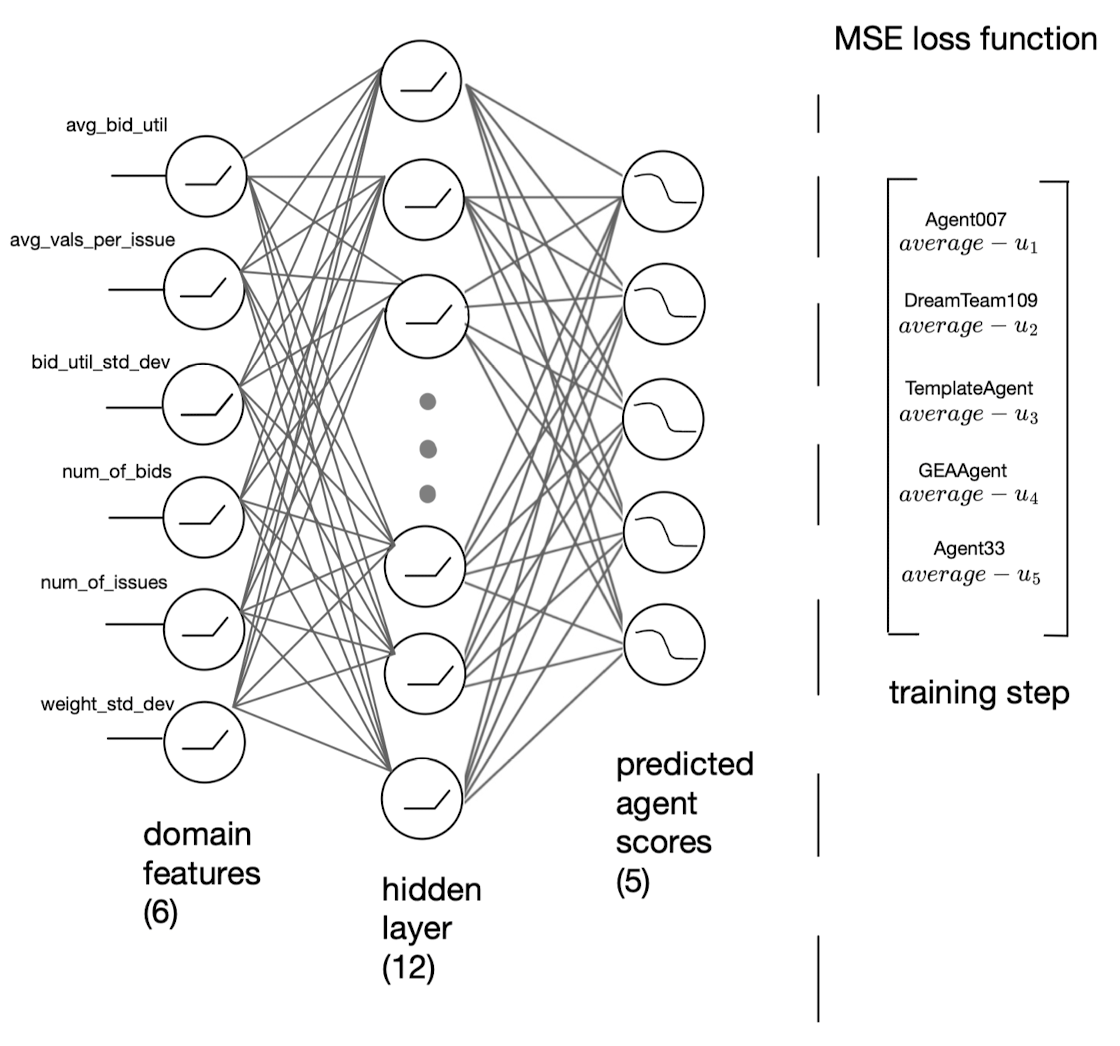
\includegraphics[scale=0.45]{nn_train.png}}
\captionsetup{justification=centering}
\caption{Neural Network Training}
\label{fig:NeuralNetworkTraining}
\end{figure}


\paragraph{}
 The Neural Network takes the domain characteristics (X) as input data along with the real average utility that the agents gained (Y) from the negotiation rounds in the specific domain. It’s goal is to train the Network (adjusting the weights and biases) so that giving the characteristics of a new domain gives us a prediction of each agent’s performance in it which can be very beneficial.  
 The training happens by passing the domain characteristics in a forwards pass, getting the outputs and using the Mean Square Error loss function to calculate the error between the outputs and the real scores and then using the optimizer, adam in our case to adjust the weights and biases with backpropagation.
 \paragraph{}
 

The architecture of the Neural Network is simple but a bit more complicated than the one decribed in the research paper \cite{meta_agent_paper}, even though not a lot of data is disclosed about it.
 We use an input layer of size 6, for each one of the domains characteristics, 
 a hidden layer of size 12 which is 2 times the size of input layer, in order to be able to detect hidden patterns in the data but showed 
 the best results between the values we tested and an output layer of size 5, for each of the agent's performance.  
 The input and hidden layers used the relu activation function and the output layer used the softmax activation function, which ensures that the outputs are a value between 0 and 1 and is a good fit for our predictions problem. We used 2 epochs for the training because it showed good results with no overfitting, like 3 or more epochs (showing similar results for different input features) and
  more effective training rounds than 1 epoch. Finally a dropout layer was applied (not shown in the figure, between the hidden layer and the output) with a dropout chance of 30\% that works by 
  randomly setting a fraction of input units to 0 at each update during training, which helps to make the model more robust and generalize better to unseen data. 
\paragraph{}



After the training is done to get the predictions for each agents, 
all we need is a forward pass of the domain characteristics from the Neural Network. 
This concludes the off-line training part of the problem, but the scope of the Negotiator does not stop there.
In the next part we test how the output of the Neural Network can give some knowledge to an on-line algorithm 
which will continue the learning with a different approach.
\begin{figure}[H]
	\centering
	\framebox{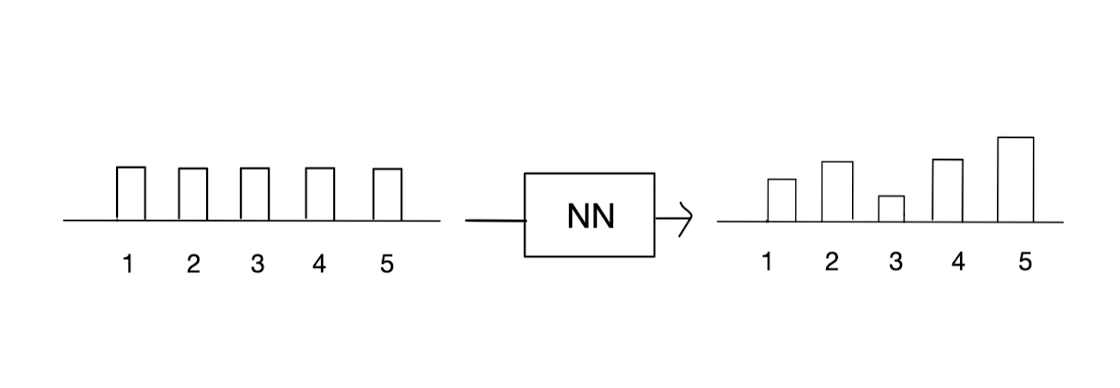
\includegraphics[scale=0.55]{nn_ucb.png}}
	\captionsetup{justification=centering}
	\caption{Setting the initial confidence bounds}
	\label{fig:Setting the initial confidence bounds}
\end{figure}
 